\chapter{Задача стабилизации с реальным дифференцирующим звеном}
Модифицируем замкнутую систему из Задания 1, заменив аппроксимацию 
производной $\dot 𝑦(𝑡)$ на передаточную функцию вида:
\[
W_{\text{p.дифф.}}(p) = \frac{p}{Tp + 1}
\]

Определить аналитически критические значения параметра $T$, при которых система
становится неустойчивой для выбранных ранее $k_0$ и $k_1$:
\[
\ddot{y} - \dot{y} + y = k_0y + k_1\dot{y}
\]
\[
\ddot{y} - \dot{y} + y = -y -3\dot{y}
\]
\[
\ddot{y} - \dot{y} + y = -y -3\frac{p}{Tp + 1}
\]

Так как для исследования устойчивости через полюсы системы, не обязательны
начальные условия, то применим преобразование Лапласа без них:
\[
    s^2 Y(s) - sY(s) + Y(s) = -Y(s) - \frac{3s}{Ts+1}
\]
\[
    s^2 - s + 1 = -1 - \frac{3s}{Ts+1}
\]
\[
    Ts^3 + s^2 - Ts^2 - s + 2Ts = -Ts - 1 - 3s
\]
\[
    Ts^3 + (1 - T)s^2 + (2T - 2)s + 2 = 0
\]

Применим критерий Гурвица:
\[
    \Delta_1 = 1 - T > 0 \Rightarrow T < 1
\]
\[
    \Delta_2 = 
    \begin{vmatrix}
        1 - T & 2 \\
        T & 2T - 2
    \end{vmatrix}
    = (1 - T)(2T - 2) - 2T = -2T^2 - 2T + 2 > 0\]
\[
    -2T^2 - 2T + 2 > 0
\]
\[
    T^2 + T - 1 < 0
\]
\[
    \frac{-1 - \sqrt{5}}{2} < T < \frac{-1 + \sqrt{5}}{2}
\]
\[
    0 < T < 0.618
\]

Выполним моделирование для $T = 0.1,\, 0.25,\, 0.45$ и сопоставим их между собой и с 
результатом моделирования замкнутой системы из Задания 1:
\begin{figure}[H]
    \centering
    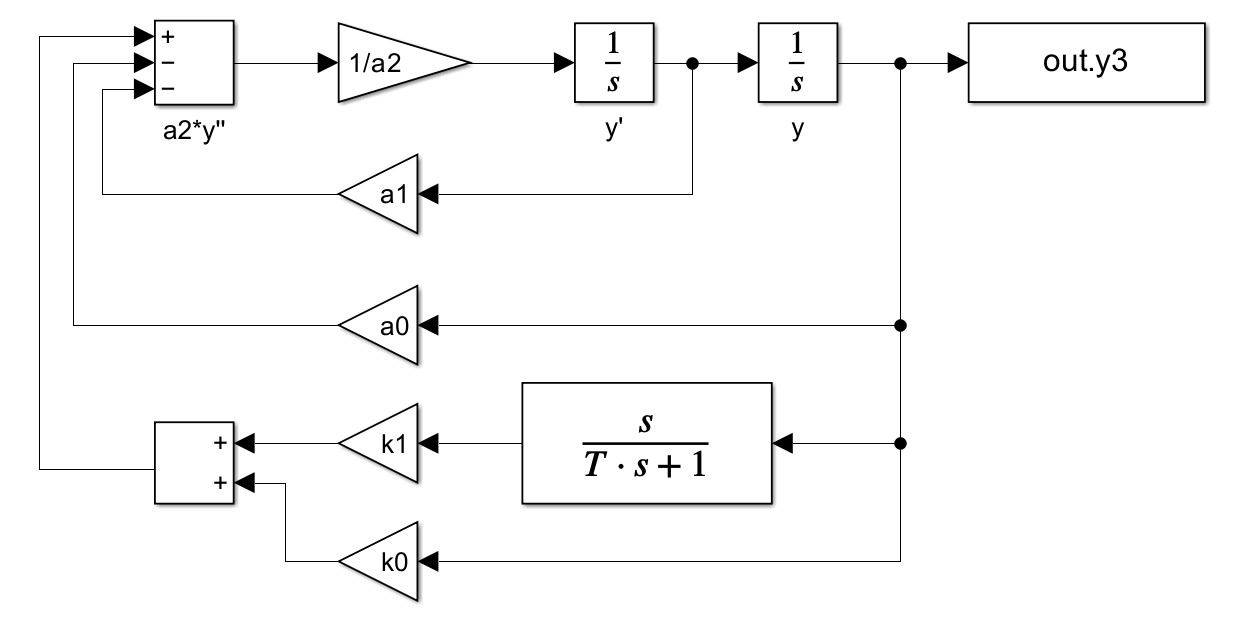
\includegraphics[width=0.8\textwidth, trim={0cm 0cm 0cm 0cm}]{../images/sim3.png}
    \caption{Схема замкнутой системы c реальным дифференцирующим звеном в Simulink}
\end{figure}
\begin{figure}[H]
    \centering
    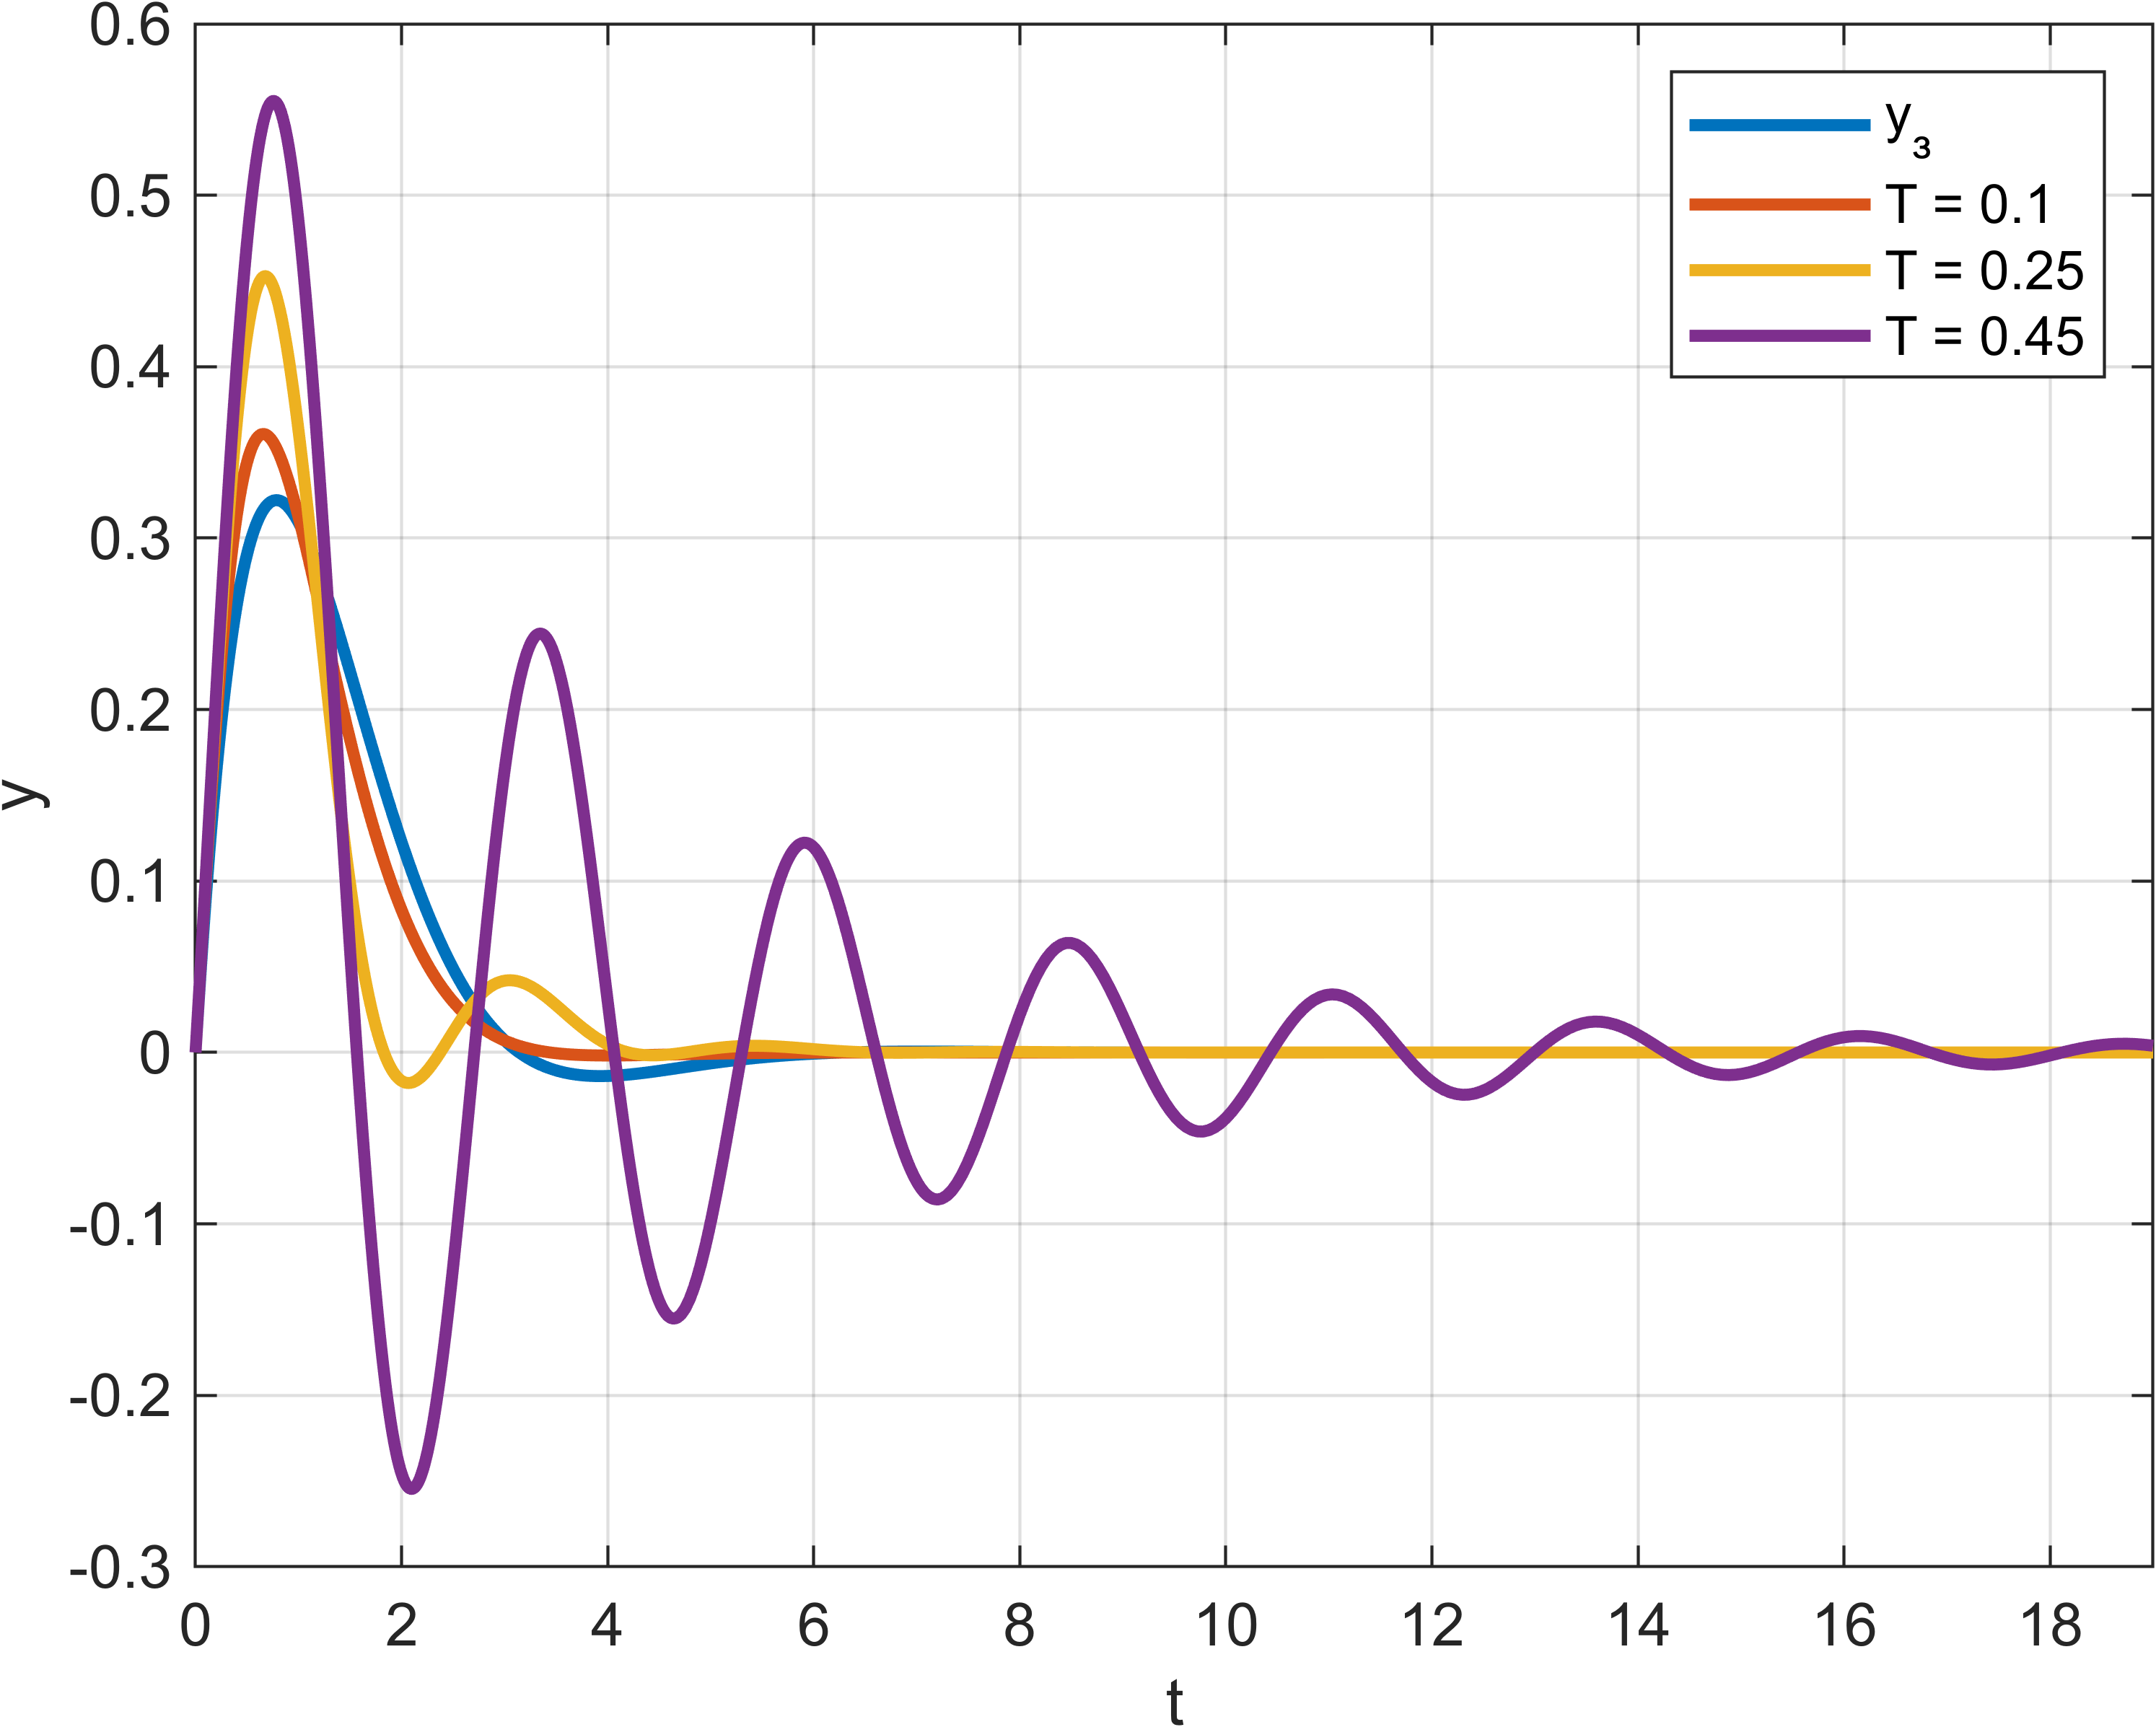
\includegraphics[width=1\textwidth, trim={0cm 0cm 0cm 0cm}]{../images/2_1.png}
    \caption{Сигналы для $T = 0.1,\, 0.25,\, 0.45$ и $y_{\text{з}}(t)$}
\end{figure}

По графикам видно, что реальное дифференцирующее звено при увеличении $T$ 
увеличивает время переходного процесса и увеличивает перерегулирование.
\endinput